\begin{ex}
Entre os 9 quadradinhos abaixo, apenas 3 devem ser pintados de vermelho e apenas 3 devem ser pintados de verde.
\begin{center}
   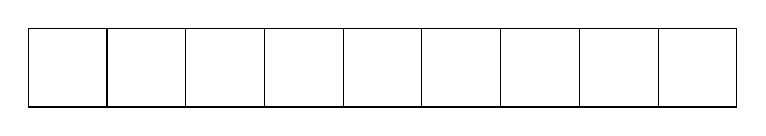
\begin{tikzpicture}
    \draw (0,0)--(9,0)--(9,1)--(0,1)--(0,0);
    \draw (1,0)--(1,1); \draw (2,0)--(2,1); \draw (3,0)--(3,1); 
    \draw (4,0)--(4,1); \draw (5,0)--(5,1); \draw (6,0)--(6,1);
    \draw (7,0)--(7,1); \draw (8,0)--(8,1); \draw (8,0)--(8,1);
   \end{tikzpicture}
\end{center}


O número de figuras diferentes que pode resultar dessa pintura é:
   \begin{enumerate}[(a)]
   \item $(3!)^3$
   \item 1680
   \item 948
   \item 2480
   \item 1400
   \end{enumerate}
      \begin{sol}
      resposta: b\\
      $\frac{9!}{3!\cdot3!\cdot3!}=1680$
      \end{sol}
\end{ex}